\lstinputlisting[language=bash,basicstyle=\small]{python_codes/fieldstone_83/keywords}

\begin{center}
Code at \url{https://github.com/cedrict/fieldstone/tree/master/python_codes/fieldstone_83}
\end{center}

\par\noindent\rule{\textwidth}{0.4pt}

{\sl This stone was developed in collaboration with Iris van Zelst}. \index{contributors}{I. van Zelst}

\par\noindent\rule{\textwidth}{0.4pt}
%%%%%%%%%%%%%%%%%%%%%%%%%%%%%%%%%%%%%%%%%%%%%%%%%%%%%%%%%%%%%%%%%%%%%%%%%%%%%%%%%%%%%%%%%%%%%%


To accurately study the thermal structure of the oceanic lithosphere, it is important to take 
into account the temperature dependence of thermal parameters such as the thermal conductivity $k$, 
heat capacity $C_p$, and the density $\rho$. Classic (analytical) models, such as the half-space 
cooling model and the plate model, typically ignore this complexity and assume constant parameters. 
Here, we model the thermal structure of oceanic lithosphere with temperature-dependent 
thermal conductivity, heat capacity, and density according to McKenzie et al. (2005) \cite{mcjp05} 
and Richards et al. (2018) \cite{rihc18}. We use a 2D approach, although there is no lateral variation, 
which essentially makes this a 1D model of cooling oceanic lithosphere with time. 
We implement various options for the temperature-dependence of the parameters (including the constant case) 
based on experimental findings and different rock compositions 
(i.e., Parsons and Slater (1977) \cite{pasc77}, 
Berman 1988, Berman and Aranovich 1996, Hofmeister 1999, Xu et al., 2004). 
We then compare our results to those of Richards et al. (2018).

We start from Eq.(1) of McKenzie et al (2005) \cite{mcjp05}:
\[
\frac{\partial}{\partial t}(\rho(T) C_p(T) T) = \vec\nabla \cdot (k(T) \vec\nabla T)
\]
Using a simple Euler scheme we have
\[
\frac{(\rho(T) C_p(T) T)^{n} - (\rho(T) C_p(T) T)^{n-1} }{\delta t} 
 = \vec\nabla \cdot (k(T^n) \vec\nabla T^n)
\]
or, 
\[
\rho(T^n) C_p(T^n) T^{n} - \delta t \vec\nabla \cdot (k(T^n) \vec\nabla T^n)
= \rho(T^{n-1}) C_p(T^{n-1}) T^{n-1} 
\]
We left multiply by a shape function $N_i$ and integrate over the whole domain $\Omega$:
\[
\int_\Omega N_i \rho(T^n) C_p(T^n) T^{n} dV-
\delta t \int_\Omega N_i \vec\nabla \cdot (k(T^n) \vec\nabla T^n) dV
= 
\int_\Omega N_i\rho(T^{n-1}) C_p(T^{n-1}) T^{n-1} dV
\]
Inside an element we have 
\[
T^h = \vec{N} \cdot \vec{T}
\]
and taking $i=1,m$ yields (see Section~\ref{ss:hte_fem})
\[
{\bm M}^n \cdot \vec{T}^n + {\bm K}^n \cdot \vec{T} ^n = \vec{f}^{n-1}
\]
with
\begin{eqnarray}
{\bm M}^n &=& \int_V \rho(T^n) C_p(T^n) \vec{N}^T \vec{N} dV  \nn\\
{\bm K}^n &=& \int_V {\bm B}^T k(T^n) {\bm B} dV \nn\\
\vec{f}^{n-1} &=& \int_V \vec{N}^T \rho(T^{n-1}) C_p(T^{n-1}) dV \nn
\end{eqnarray}
The second term has been integrated by parts (and the surface term disregarded:
Dirichlet boundary conditions top and bottom, and zero heat flux on the sides).


The density is given by Eq.(9) of \cite{mcjp05}:
\begin{equation}
\rho(T)=\rho_0 \exp -\left[\alpha_0 (T-273) + \frac{\alpha_1}{2} (T^2-273^2) \right]
\label{eq:f83_1}
\end{equation}
with $\rho_0=3330\si{\kg\per\cubic\meter}$.

The heat capacity is given by Eq.(10) of \cite{mcjp05}:
\begin{equation}
C_p(T) = k_0 + k_1 T^{-1/2} + k_3 T^{-3}
\label{eq:f83_2}
\end{equation}
with $k_0=233.18$, $k_1=-1801.6$ and $k_3=-26.794\cdot 10^{7}$ for fosterite and 
$k_0=252$, $k_1=-2013.7$ and $k_3=-6.219\cdot10^{7}$ for fayalite. We assumed that the
molar fraction of fayalite in the mantle is 11\%. 

The heat conductivity is given by Eq.(4) of \cite{mcjp05}:
\begin{equation}
k(T)=\frac{b}{a+cT} + \sum_{m=0}^3 d_m (T+273)^m
\label{eq:f83_3}
\end{equation}
with $b=5.3$, $c=0.0015$, $d_0=1.753\cdot10^{-2}$, $d_1=-1.0365\cdot10^{-4}$, $d_2=2.2451\cdot10^{-7}$ and 
$d_3=-3.4071\cdot10^{-11}$


Because the coefficients $\rho(T)$, $C_p(T)$ and $k(T)$ depend on the temperature, which is the unknown 
of the PDE, this PDE is highly nonlinear and a dedicated algorithm {\it should} then be designed to handle the 
nonlinearity. For now the code disregards those considerations and its structure is identical to the linear equation case.

Following Richards et al, we run the model for 170Myr. Boundary conditions are $T=0\si{\celsius}$ 
at the top and $T=1350\si{\celsius}$ at the bottom. The functions for $k(T)$, $C_p(T)$ and $\rho(T)$
are in a separate file {\sl temperature\_dependent\_variables.py}.

%.....................................
\subsection*{Constant parameters}

In this case we set $k=3.138$, $C_p=1171.52$ and $\rho=3330$.


\begin{center}
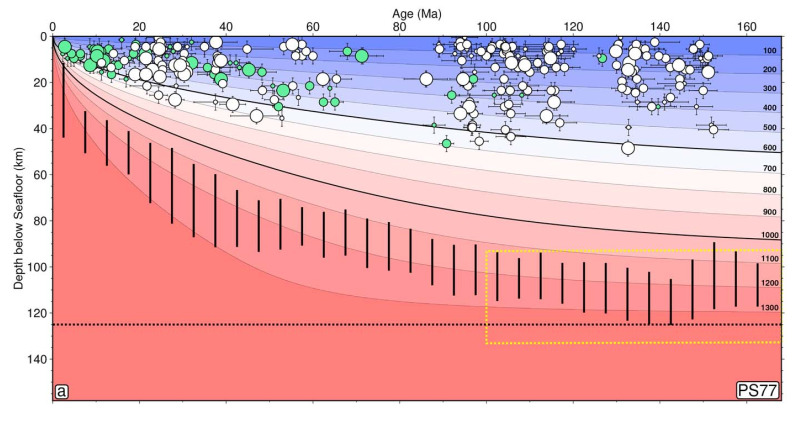
\includegraphics[width=12cm]{python_codes/fieldstone_83/images/rihc18a}\\
{\captionfont Taken from Richards et al (2018) \cite{rihc18}.
Thermal structure of oceanic lithosphere. 
(a) Simple analytical plate model using the published values reported by Parsons and Sclater (1977) \cite{pasc77}; 
numbered contours = isothermal surfaces plotted in \si{\celsius}; 
green and white circles with error bars = oceanic intraplate and outer rise earthquakes 
from Craig et al. (2014) where small/medium/large circles 
= $M_b < 5.5$, $5.5-6.5$, and $> 6.5$; 
vertical black bars = depth to lithosphere-asthenosphere boundary in the Pacific Ocean
based upon peak variations in azimuthal anisotropy (Burgos et al., 2014); 
dashed box = envelope of depths to lithosphere-asthenosphere boundary for plate 
ages $>100$ Ma (Steinberger \& Becker (2018) \cite{stbe18}); 
horizontal black dashed line = base of plate model. 
} 
\end{center}

\begin{center}
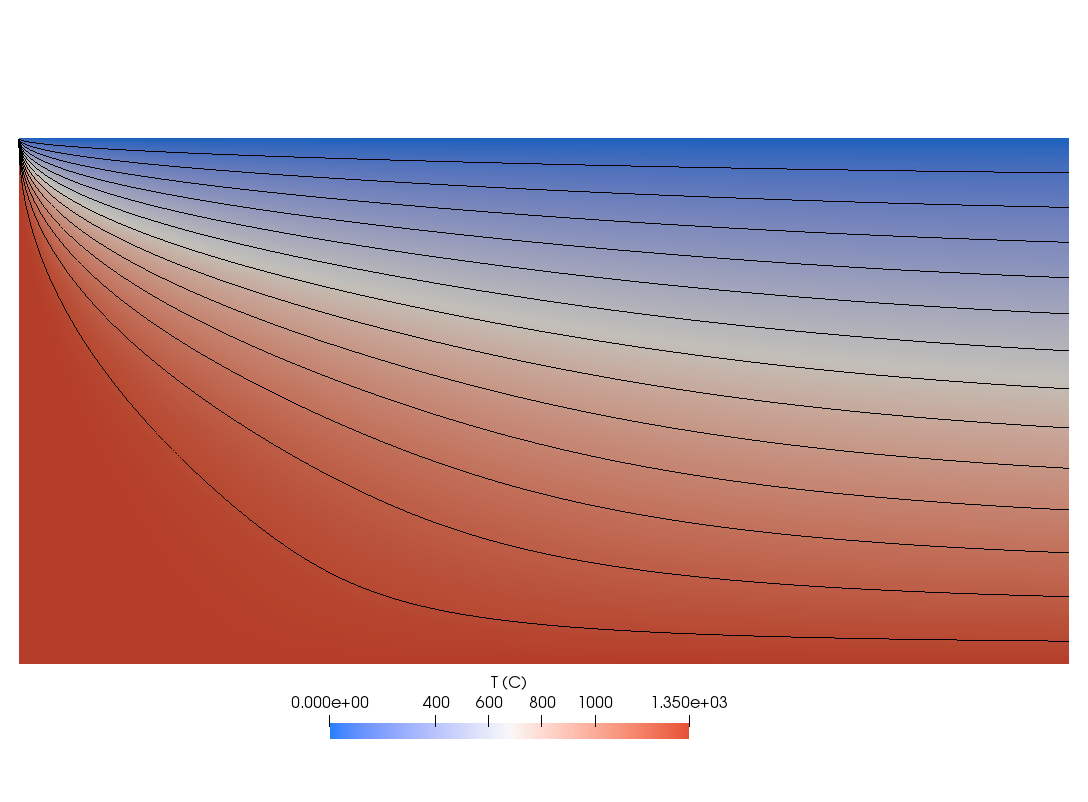
\includegraphics[width=7cm]{python_codes/fieldstone_83/results_model1/T}
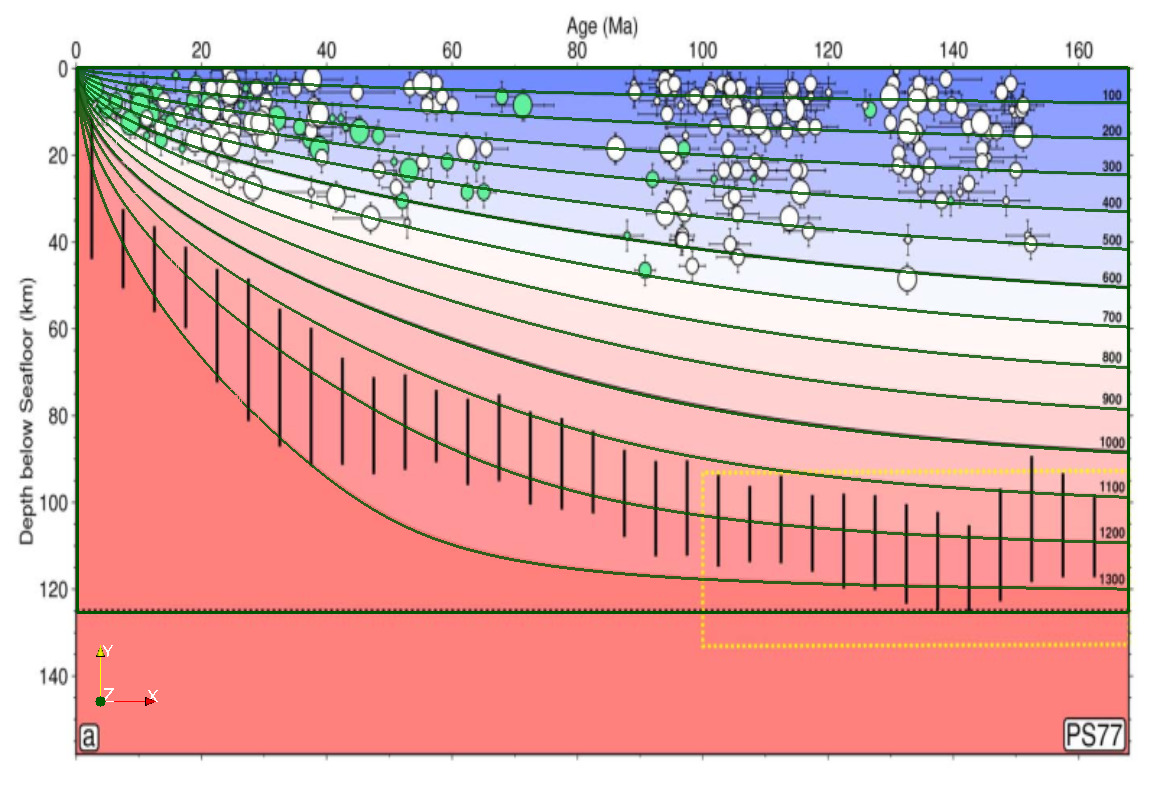
\includegraphics[width=7cm]{python_codes/fieldstone_83/results_model1/comparison}\\
{\captionfont Isocontours every 100$\si{\celsius}$ between 0 and 1300.}
\end{center}

\begin{center}
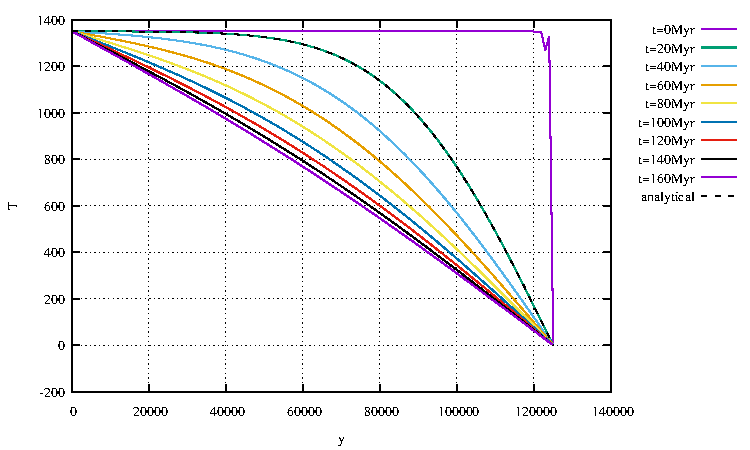
\includegraphics[width=10cm]{python_codes/fieldstone_83/results_model1/Tprofiles}\\
{\captionfont Temperature profile evolution.} 
\end{center}



%.....................................
\subsection*{T-dependent parameters a la McKenzie et al (2015)}

\begin{center}
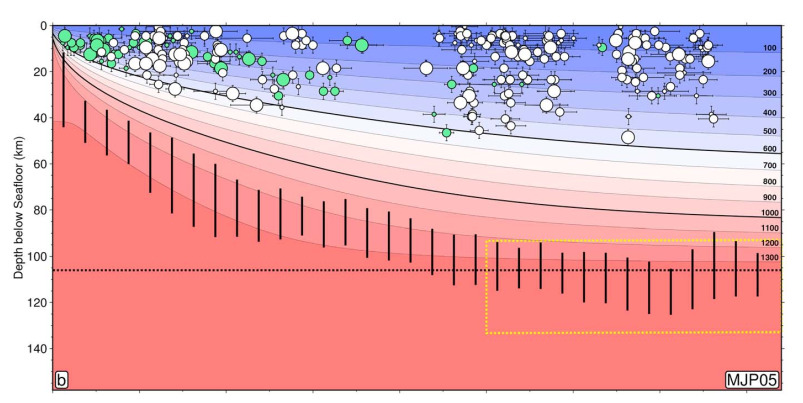
\includegraphics[width=12cm]{python_codes/fieldstone_83/images/rihc18b}\\
{\captionfont Same for the purely temperature-dependent plate model using parameter values from
McKenzie et al. (2005) \cite{mcjp05}.}
\end{center}

\begin{center}
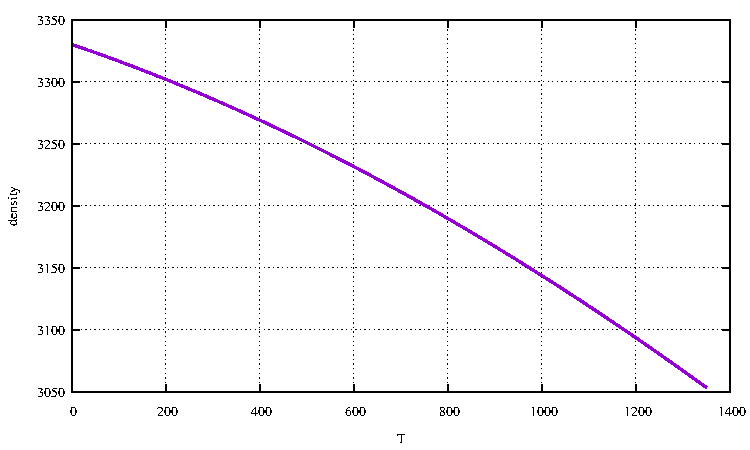
\includegraphics[width=5cm]{python_codes/fieldstone_83/results_model2/rho.pdf}
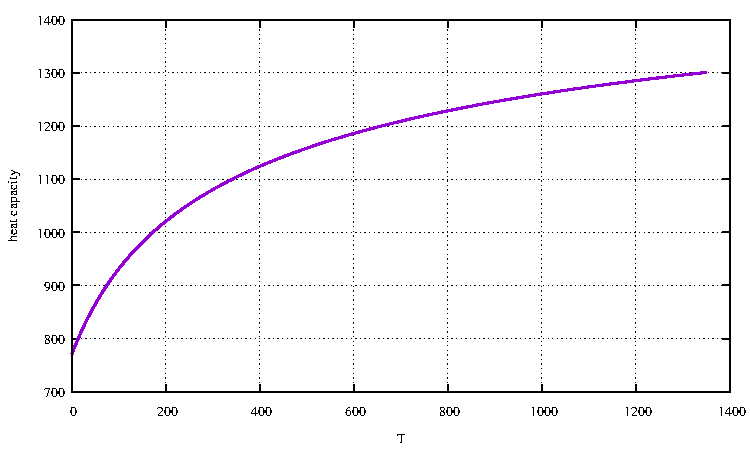
\includegraphics[width=5cm]{python_codes/fieldstone_83/results_model2/hcapa.pdf}
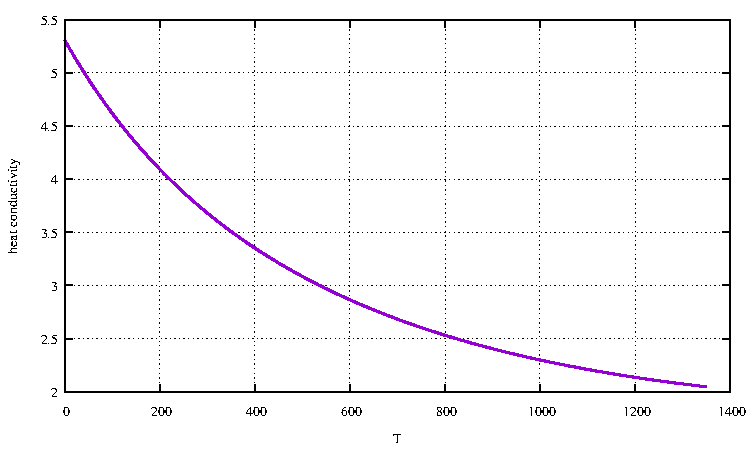
\includegraphics[width=5cm]{python_codes/fieldstone_83/results_model2/hcond.pdf}\\
{\captionfont Density, heat capacity and heat conductivity as obtained from Eqs.~\eqref{eq:f83_1}, \eqref{eq:f83_2}, and \eqref{eq:f83_3}.}
\end{center}


\begin{center}
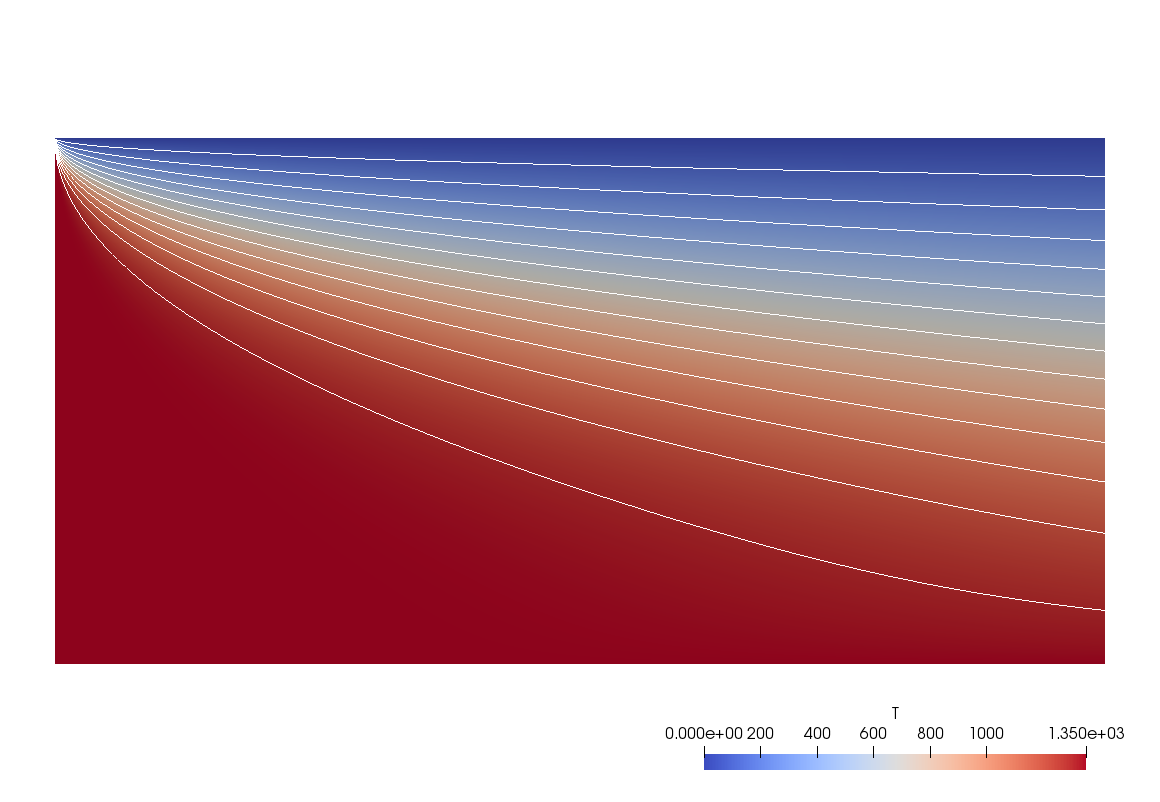
\includegraphics[width=7cm]{python_codes/fieldstone_83/results_model2/T}
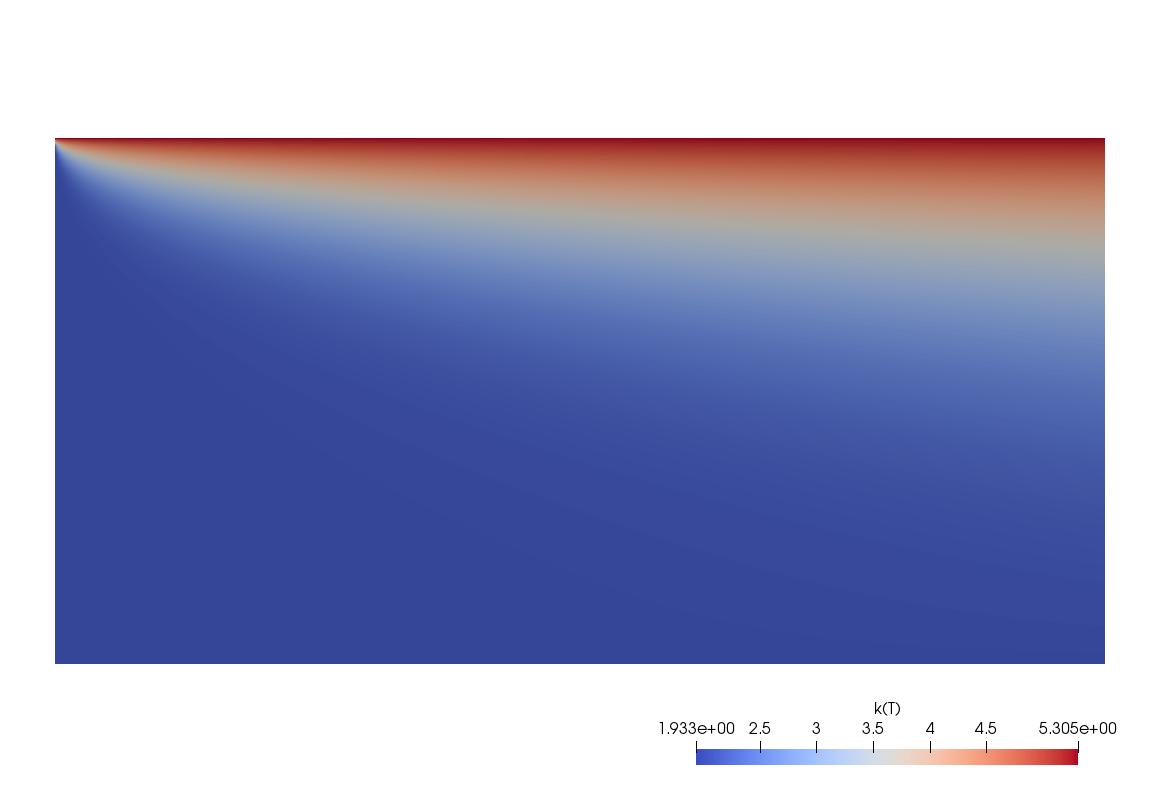
\includegraphics[width=7cm]{python_codes/fieldstone_83/results_model2/k}\\
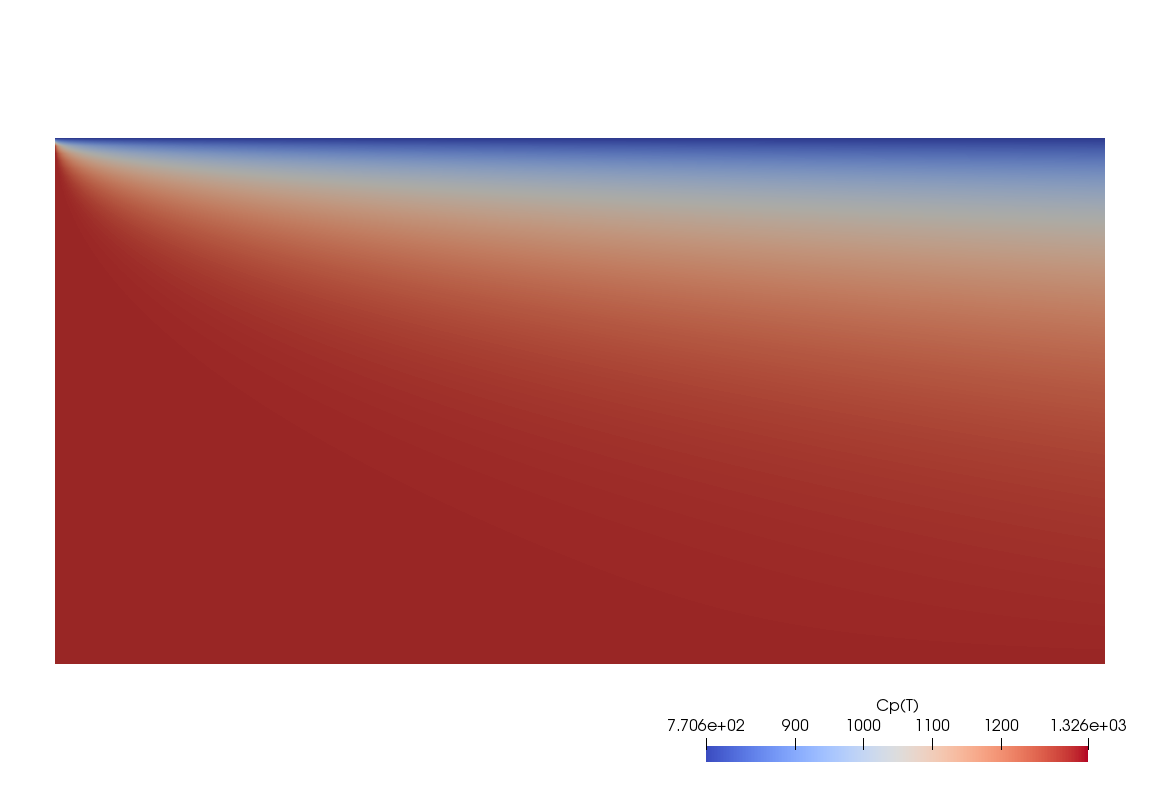
\includegraphics[width=7cm]{python_codes/fieldstone_83/results_model2/Cp}
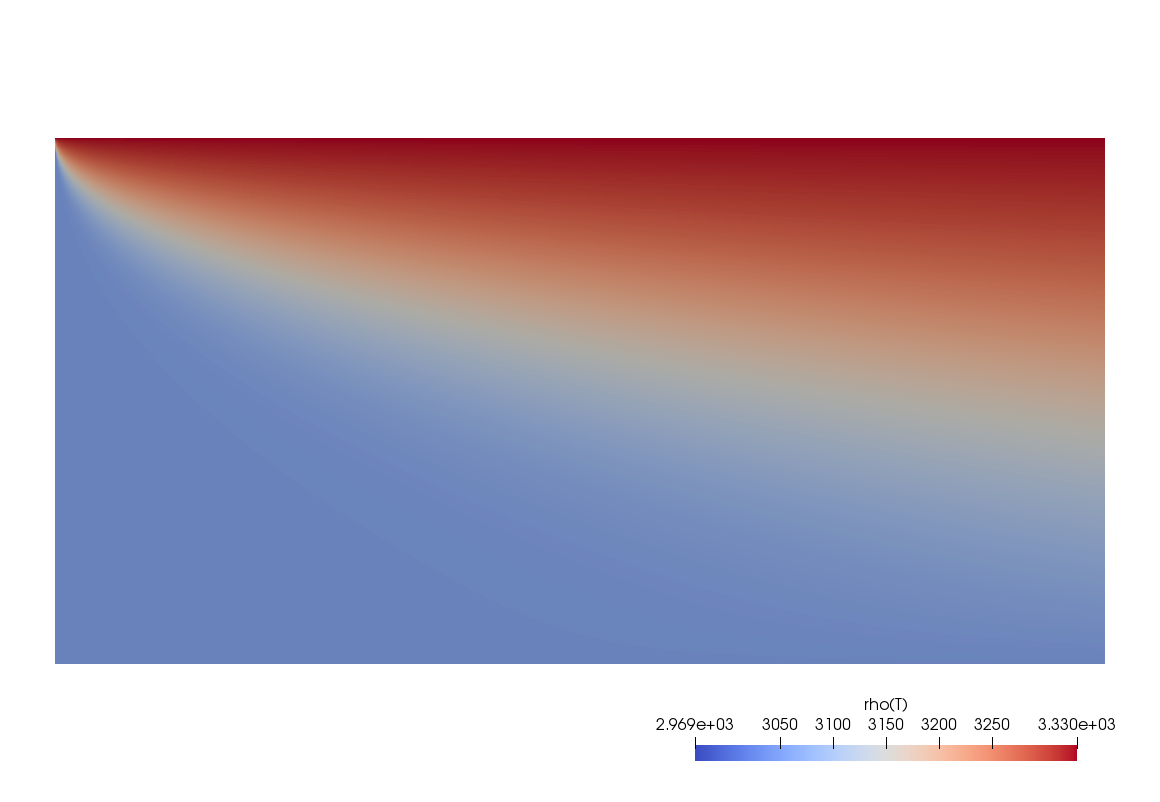
\includegraphics[width=7cm]{python_codes/fieldstone_83/results_model2/rho.png}\\
{\captionfont RERUN}
\end{center}

\begin{center}
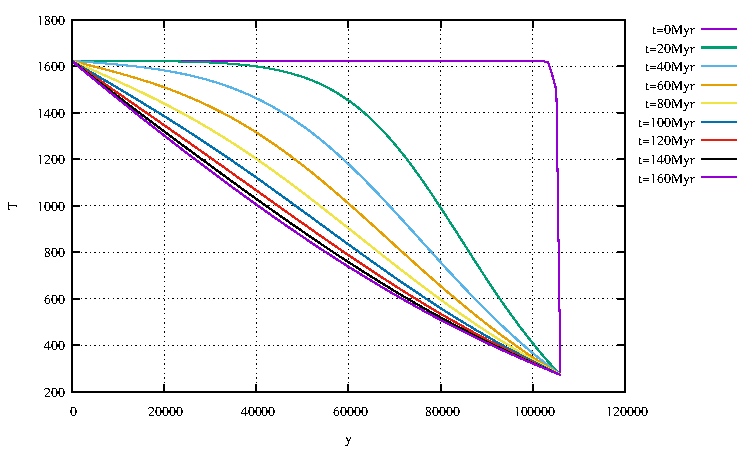
\includegraphics[width=10cm]{python_codes/fieldstone_83/results_model2/Tprofiles}\\
{\captionfont Temperature profile evolution.}
\end{center}


